\section{Design of CFA}
\label{sec:cfa:design}

In this section, we present the detailed design of \dda 
and discuss how we address the two practical challenges 
mentioned in the previous section: learning critical features 
and reducing update delay.

The key  to addressing these challenges
%,  which leads 
% to the practical realization of \dda, 
 is our third and final domain-specific insight:

\begin{insight}
Critical features tend to {\em persist} on long timescales
of tens of minutes.
\label{insight:persistence}
\end{insight}

 This insight is derived from prior measurement 
 studies.
 For instance, our measurement study in 
 Chapter~\ref{ch:measurement} 
 on shedding light on video quality issues in the wild showed 
 that the factors that lead to poor video quality persist
 for hours, and sometimes even days.  
 Another recent study from the C3 system suggests that 
 the best CDN tends to be relatively stable on the 
 timescales of few tens of minutes~\cite{c3}.  
We independently confirm this observation in 
Section~\ref{subsec:eval-scalability} that 
using slightly stale critical features (e.g., 30-60 minutes 
 ago) achieves similar prediction accuracy as using the 
most up-to-date critical features.
Though this insight holds for most cases, it is still possible
(e.g., on mobile devices) that critical features persist on a 
relatively shorter timescale (e.g., due to the nature of 
mobility).
%For instance, on a mobile device, the persistency of critical features
%might be shorter than tens of minutes due to the nature of mobility.}


% we show that using slightly stale 
%^critical features (i.e., learned 30-60 minutes ago) achieves
%s%imilar prediction accuracy as using the most up-to-date 
%c%ritical features, suggesting that the persistence of critical 
%features is on timescale of tens of minutes.

Note that the persistence of critical features does not 
mean that quality values are equally persistent.  
In fact, persistence of critical features is on a 
timescale an order of magnitude longer than 
the persistence of quality.  
That is, even if quality fluctuates rapidly, the critical 
features that determine the quality do not change 
as often.


As we will see below, this persistence enables 
(a) automatic learning  of critical features from history, 
and (b) a scalable workflow that provides 
up-to-date estimates. 


\subsection{Learning Critical Features}
\label{subsec:cfa:design:learning}

Recall that the first challenge is
% that we cannot statically map each
%session to its critical features 
obtaining the critical features for each session.
The  persistence of  critical features has a natural 
corollary that we can use to automatically learn them: 

\begin{imp}
Persistence  implies that 
critical features of a session are learnable from history.
\label{imp:learning}
\end{imp}

%The key notation is {\em \HSimSessSet}
%$\HSimilarSessionSet{\HSession}{\HSessionSet}{\HFeatureSet}{\HTimeWindow}$, which consists of sessions in $\HSessionSet$ that match $\HSession$ on features in $\HFeatureSet$ and happened within time window $\HTimeWindow$ before $\HSession$. 
%For instance, $\HSimilarSessionSet{\HSession}{\HSessionSet}{\{CDN\}}{\textrm{5 minutes}}$ 
%includes all sessions that use same CDN with $\HSession$ 
%and happened within 5 minutes before $\HSession$. 
%Note that, prediction made by Algorithm~\ref{alg:critical-feature} is 
%$\HPred{\HSession}{\HSessionSet}=\HEst{\HSimilarSessionSet{\HSession}{\HCriticalFeature{\HSession}}{\HFeatureSet}{\HTimeWindow}}$.


\begin{table}[t!]
%\begin{footnotesize}
\begin{tabular}{p{3.5cm}|p{3cm}|p{7.5cm}}
{\bf Notations} & {\bf Domains} & {\bf Definition} \\ \hline\hline
$\HSession,\HSessionSet,\HSessionFullSet$ & & A session, a set of sessions, set of all sessions \\ \hline
%$\HSession$ & & A video session \\ \hline
%$\HSessionSet$ & & A set of video sessions \\ \hline
%$\HSessionFullSet$ & & Set of all video sessions \\ \hline
%$\HSessionTime{\HSession}$ & $\HSessionFullSet\mapsto\HReal$ & Timestamp of $\HSession$ \\ \hline
$\HSessionQuality{\HSession}$ & $\HSessionFullSet\mapsto\HReal$ & Quality of $\HSession$ \\ \hline
$\HDistribution{\HSessionSet}$ & $2^\HSessionFullSet\mapsto2^\HReal$ & $\{\HSessionQuality{\HSession}|\HSession\in\HSessionSet\}$ \\ \hline
%$\HEst{\HSessionSet}$ & $2^\HSessionFullSet\mapsto\HReal$ & Summarizing value (by default, median) of $\HDistribution{\HSessionSet}$ \\ \hline
%$\HDist{\HSessionSet_1}{\HSessionSet_2}$ & $2^\HSessionFullSet\times2^\HSessionFullSet\times\HReal$ & JS divergence of $\HDistribution{\HSessionSet_1}$ and $\HDistribution{\HSessionSet_2}$\\ \hline
$\HFeature,\HFeatureSet,\HFeatureFullSet$ & & A feature, a set of features, set of all features \\ \hline
%$\HFeature$ & & A session feature \\ \hline
%$\HFeatureSet$ & & A set of session features \\ \hline
%$\HFeatureFullSet$ & & Set of all session features \\ \hline
$\HCriticalFeature{\HSession}$ & $\HSessionFullSet\mapsto2^\HFeatureFullSet$ & Critical features of $\HSession$ \\ \hline
$\HFeatureValueFullSet$ & & Set of all feature values \\ \hline
$\HFeatureValue{\HFeature}{\HSession}$ & $\HFeatureFullSet\times\HSessionFullSet\mapsto\HFeatureValueFullSet$ & Value on feature $\HFeature$ of $\HSession$ \\ \hline
$\HFeatureSetValue{\HFeatureSet}{\HSession}$ & $2^\HFeatureFullSet\times\HSessionFullSet\mapsto2^\HFeatureValueFullSet$ & Set of values on features in $\HFeatureSet$ of $\HSession$ \\ \hline
$SimilarSessionSet$ $(\HSession,\HSessionSet,\HFeatureSet,\HTimeWindow)$ & $\HFeatureFullSet\times2^\HFeatureFullSet\times\HSessionFullSet\times\HReal^{+}\mapsto2^\HFeatureFullSet$ & $\{\HSession'|\HSession'\in\HSessionSet,\HSessionTime{\HSession}-\HTimeWindow<\HSessionTime{\HSession'}<\HSessionTime{\HSession},\HFeatureSetValue{\HFeatureSet}{\HSession'}=\HFeatureSetValue{\HFeatureSet}{\HSession}\}$ \\ 
%\hline
%$\HPred{\HSession}{\HSessionSet}$ & $\HSessionFullSet\times2^\HSessionFullSet\mapsto\HReal$ & Prediction function
\end{tabular}
%\end{footnotesize}
\caption{Notations used in learning of critical features.}
\label{tab:terminology}
%\vspace{-0.5cm}
\end{table}



Specifically, we can simply look back over the history and identify  
the subset of features $\HFeatureSet$ such that the quality 
distribution of sessions matching on $\HFeatureSet$ is most similar 
to that of sessions matching on {\em all} features.   
For instance, suppose we have three features
$\langle \mathit{ContentName},\mathit{ASN},\mathit{CDN}\rangle$ and 
it turns out that sessions with  $\mathit{ASN}=\mathit{Comcast},
\mathit{CDN}=\mathit{Level3}$ consistently
have  high buffering over the last few hours due to some internal 
congestion at the corresponding exchange point. 
Then, if we look back over the last few hours, the data from 
history will   naturally reveal  that the distribution of the quality of 
sessions  with the feature values
$\langle\mathit{ContentName}=\mathit{Foo},
\mathit{ASN}=\mathit{Comcast},\mathit{CDN}=\mathit{Level3}\rangle$
will be  similar to $\langle \mathit{ContentName}=\mathit{*},
\mathit{ASN}=\mathit{Comcast},\mathit{CDN}=\mathit{Level3} \rangle$, 
but very different from, say, the quality of sessions in 
$\langle \mathit{ContentName}=\mathit{*},\mathit{ASN}=\mathit{*},
\mathit{CDN}=\mathit{Level3} \rangle$,
or $\langle \mathit{ContentName}=\mathit{*},
\mathit{ASN}=\mathit{Comcast},\mathit{CDN}=\mathit{*} \rangle$.
Thus, we can use a data-driven approach to learn that 
$\mathit{ASN},\mathit{CDN}$ are the critical features for sessions 
matching $\langle \mathit{ContentName}=\mathit{Foo},
\mathit{ASN}=\mathit{Comcast},\mathit{CDN}=\mathit{Level3} \rangle$.




% irrespective  of other feature values, sessions wit history that predicting the quality 
  



%Inspired by \impref{imp:learning}, we learn critical features 
%over a time window, during which critical features persist. 
%Intuitively, critical features are the subset of features 
%that meet two requirements.
%\begin{packeditemize}
%\item First, there should enough sessions
%for quality estimation of Algorithm~\ref{alg:critical-feature}
%to avoid unreliable prediction due to curse of dimensionlity.
%This is guaranteed by line 7-9.
%\item Second, among subsets of features that meet the first 
%requirement, we find the subset of features $\HFeatureSet$ such that 
%quality distribution of sessions matching $\HFeatureSet$ is the 
%most similar to that of sessions matching all features
%, 
%because these two sets of sessions should be determined by 
%the same set of critical features.
%\end{packeditemize}
%Finally, we should take into account two key aspects of model 
%expressiveness (\Section\ref{subsec:expressive}):
%high diversity (critical features are learned for each session 
%under prediction), and high dimensionality (critical features could be 
%any subsets of features). 


\begin{algorithm}[t!]
\begin{small}
 \KwIn{Session under prediction \HSession, Previous sessions \HSessionSet}
 \KwOut{Critical features for  \HSession}
 \tcc{Initialization}
 $\mathit{MaxSimilarity}\leftarrow-\infty,\mathit{CriticalFeatures}\leftarrow \mathit{NULL}$\;
 %\tcc{$D_{finest}$:Quality distribution of \HSimilarSessionSet{\HSession}{\HSessionSet}{\HFeatureFullSet}{\HTimeWindowLearn}.}
 \tcc{$D_{finest}$:Quality distribution of sessions matching on $\HFeatureFullSet$ in $\HTimeWindowLearn$.}
 $D_{finest}\leftarrow\HDistribution{\HSimilarSessionSet{\HSession}{\HSessionSet}{\HFeatureFullSet}{\HTimeWindowLearn}}$\;
 \For{$\HFeatureSet\subseteq2^\HFeatureFullSet$}{
	\tcc{Exclude $\HFeatureSet$ without enough similar sessions for prediction.}
	\If{$|\HSimilarSessionSet{\HSession}{\HSessionSet}{\HFeatureSet}{\HTimeWindowEst}|<n$}{{\bf continue\;}}
 	%\tcc{$D_{\HFeatureSet}$:Quality distribution of \HSimilarSessionSet{\HSession}{\HSessionSet}{\HFeatureSet}{\HTimeWindowLearn}.}
	\tcc{$D_{\HFeatureSet}$:Quality distribution of sessions matching on $\HFeatureSet$ in $\HTimeWindowLearn$.}
	$D_{\HFeatureSet}\leftarrow\HDistribution{\HSimilarSessionSet{\HSession}{\HSessionSet}{\HFeatureSet}{\HTimeWindowLearn}}$\;
	\tcc{Get similarity of $D_{finest}$ \& $D_{\HFeatureSet}$.}
	$\mathit{Similarity}\leftarrow\HDist{D_{\HFeatureSet}}{D_{finest}}$\; 	\If{$\mathit{Similarity}>\mathit{MaxSimilarity}$}{
		$\mathit{MaxSimilarity}\leftarrow \mathit{Similarity}$\;
		$\mathit{CriticalFeatures}\leftarrow \HFeatureSet$\;
	}
 }
 \Return{CriticalFeature}\;
\end{small}
 \caption{{\bf {\em Learning of critical features.}}}
\label{alg:learning}
\end{algorithm}

Algorithm~\ref{alg:learning}  formalizes this intuition for learning 
critical features. 
Table~\ref{tab:terminology} summarizes the notation used in
Algorithm~\ref{alg:learning}.
For each subset of features $\HFeatureSet$ (line 3), 
we compute the similarity between the quality distribution 
($D_{\HFeatureSet}$) of sessions matching on $\HFeatureSet$ 
and the quality distribution ($D_{finest}$) of sessions
matching on all features (line 7). 
% \vyas{please refer to the pseudocode in the text with the line numbers etc. dont just 
%assume ppl will read pseudocode and follow!!}
Then, we find the $\HFeatureSet$ that yields the maximum 
similarity (line 8-10), under one additional constraint that 
$\HSimilarSessionSet{\HSession}{\HSessionSet}{\HFeatureSet}{\HTimeWindowEst}$ 
should include enough (by default, at least 10) sessions to get 
reliable quality estimation (line 4-5).
%there
%should be enough sessions to  get reliable quality
%estimates, i.e., $\HSimilarSessionSet{\HSession}{\HSessionSet}{\HFeatureSet}{\HTimeWindowEst}$
%needs to have at least $n$ (by default, 10) sessions (line 4-5).
This check ensures that the algorithm will not simply return the set of all features.



As an approximation of the duration in which critical features 
persist, we use $\HTimeWindowLearn=60min$.
Note that $\HTimeWindowLearn$ is an order of magnitude 
larger than the time window $\HTimeWindowEst$ used in 
quality estimation, because critical features persist on a 
much longer timescale than quality values.
%Default value of $n$ is 10 sessions. 
We use (the negative of) Jensen-Shannon 
divergence between $D_1$ and $D_2$ to quantify their 
similarity $\HDist{D_1}{D_2}$.
%(assuming both of them are draw from a normal distribution).





Although Algorithm~\ref{alg:learning} can handle most cases, 
there are corner cases where
$\HSimilarSessionSet{\HSession}{\HSessionSet}
{\HFeatureFullSet}{\HTimeWindowLearn}$ 
does not have enough sessions (i.e., more than $n$) to 
%learn $\HCriticalFeature{\HSession}$ reliably. 
compute $\HDist{D_{\HFeatureSet}}{D_{finest}}$ reliably. 
In these cases, we replace $D_{finest}$ by the set of $n$ 
sessions that share most features with $\HSession$ 
over the time window of $\HTimeWindowLearn$. 
Formally, we use 
$\{\HSession'|\HSession'\textrm{ matches $k_{\HSession}$ 
features with }\HSession\}$, 
where $k_{\HSession}=\argmin_k\left(|\{\HSession'|\HSession'\textrm{ matches $k$ features with }\HSession\right|\geq n\}|)$.





\subsection{Using Fresh Updates}
\label{subsec:scalability}

Next, we focus on reducing the update delay
between when a quality measurement is received and 
used for prediction. 



Naively running critical feature learning and quality 
estimation of Algorithm~\ref{alg:critical-feature}
can be time-consuming, causing the predictions to 
rely on stale data.
In Figure~\ref{fig:scalable-workflow}(a), $T_{CFL}$ and 
$T_{QE}$ are the duration of critical feature learning and 
the duration of quality estimation, respectively. 
The staleness of quality estimation (depicted in 
Figure~\ref{fig:scalable-workflow}) 
to respond to a prediction query can be as large as the 
total time of two steps (i.e., $T_{CFL}+T_{QE}$), which 
typically is tens of minutes 
(Section~\ref{subsec:eval-scalability}).
%This is because the critical feature learning (line 1) typically takes tens of 
%minutes to update its results (\Section\ref{subsec:eval-scalability}).
%To see why, consider Figure~\ref{fig:scalable-workflow}(a), where $T_{CFL}$ and $T_{QE}$ are the duration
%of critical feature learning and the duration of quality estimation, respectively. 
%To respond a prediction query, the staleness of quality estimation is up to the total time 
%of two steps (i.e., $T_{CFL}+T_{QE}$).
Also, simply using more parallel resources is not sufficient. 
The time to learn critical features using
Algorithm~\ref{alg:learning} grows linearly with the number of 
sessions under prediction, the number of history sessions,
and the number of possible feature combinations.
Thus, the complexity of learning critical features $T_{CFL}$ is 
exponential in the number of features. Given the current 
set of features, $T_{CFL}$ is on the scale of tens of minutes.

%This means the complexity of learning critical features is 
%super-linear to the size of data (number of sessions and 
%number of available features). Thus, simply adding more 
%resources will not suffice.

\begin{figure}[t!]
\centering
%\vspace{-0.3cm}
%\hspace{-0.6cm}
%\subfigure[Naive workflow]
%{
%\includegraphics[width=0.25\textwidth]{figures/scalability-naive.pdf}
%\label{subfig:scalability-naive}
%}
%\hspace{-0.4cm}
%\subfigure[CFA workflow]
%{
%\includegraphics[width=0.25\textwidth]{figures/scalability-cfa.pdf}
%\label{subfig:scalability-cfa}
%}
%\hspace{-0.6cm}
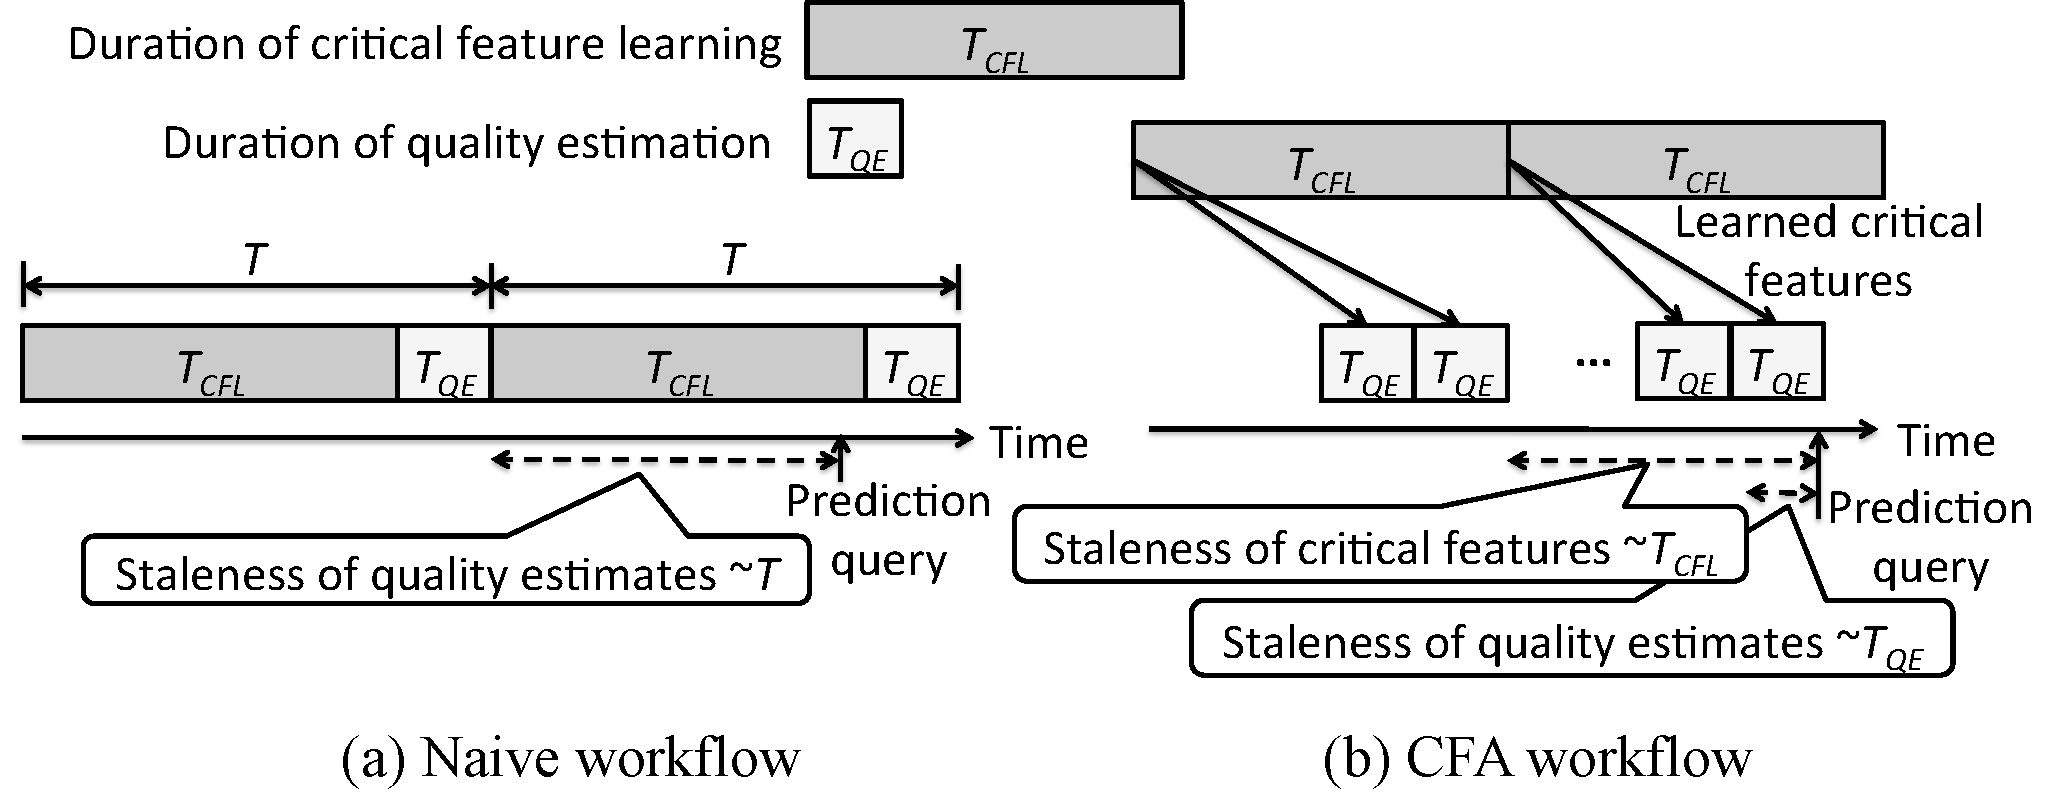
\includegraphics[width=0.9\textwidth]{figures/cfa-scalability-naive-cfa.pdf}
\caption{To reduce update delay, we run critical feature learning 
and quality estimation at different timescales by leveraging 
persistence of critical features.}
\label{fig:scalable-workflow}
\end{figure}

To reduce update delay, we again leverage the 
persistence of critical features:

\begin{imp}
Persistence implies that critical features can be cached and reused
 over tens of minutes.
\label{imp:reducing}
\end{imp}


 Building on \impref{imp:reducing}, we decouple the 
critical feature learning and quality estimation steps, and run
them at separate timescales.
On the timescale of tens of minutes, we update the results of 
critical feature learning. Then, on a faster timescale of tens of seconds, 
we update quality estimation using fresh data and the most recently
learned critical features. 

This decoupling 
%ensures that each step 
%can update its result sufficiently frequently to 
minimizes the impact of staleness on prediction accuracy.
Learning critical features on the timescale of tens 
of minutes
%\camera{\footnote{Learning critical features on a much larger set of features could take longer, 
%but it is enough for the current set of features, and the feature set will not grow very quickly.}}
is sufficiently fast as they persist 
on the same timescale.
%Since critical features persist, learning them
%on the timescale of tens of minutes is sufficient to capture their dynamics.
Meanwhile, %based on learned critical features, 
quality estimation can be updated every tens of seconds 
and makes predictions based on quality updates with sufficiently
low staleness.
Thus, the staleness of quality estimation $T_{QE}$ of
the decoupled workflow (Figure~\ref{fig:scalable-workflow}(b))
is a magnitude lower than $T_{QE}+T_{CFL}$ of the naive workflow 
(Figure~\ref{fig:scalable-workflow}(a)).
In Section~\ref{subsec:eval-scalability}, we show that 
this workflow can retain the freshness of critical features and quality estimates.
%\camera{It should be noticed that, though $T_{QE}+T_{CFL}$ (tens of minutes) 
%is not long enough to handle any number of features, 
%it is enough for \dda to learn critical features from the current feature set, 
%and the feature set will not grow very quickly.}


In addition, \dda has a natural property that two sessions sharing 
all feature values and occurring close in time will map to the 
same critical features. Thus, instead of running the steps 
per-session, we can reduce the computation to the granularity of 
{\em \leafs}, i.e., distinct values of all features.


\subsection{Putting It Together}

Building on these insights, we create 
the following practical {\em three-stage} workflow of \dda.

\begin{packeditemize}

\item {\bf Stage I: Critical feature learning} 
(line 1 of Algorithm~\ref{alg:critical-feature}) runs offline, say, 
every tens of minutes to an hour.  The output of this stage is a 
key-value table called {\em critical feature function} that maps 
all observed \leaf{s} to their critical features.

\item {\bf Stage II: Quality estimation} 
(line 2,3 of Algorithm~\ref{alg:critical-feature}) runs every tens of seconds 
for all observed \leafs based on the most recent critical features 
learned in the first stage.  
This outputs another key-value table called {\em quality function}
that maps a \leaf to the quality estimation, by aggregating the most 
recent sessions with the corresponding critical features.


\item {\bf Stage III: Real-time query/response.} Finally, we 
provide real-time query/response on the arrival of each client,
operating  at the millisecond timescale, by simply looking up the 
most recent precomputed value function from the previous stage.  
These operations are simple and can be done very fast.

\end{packeditemize}
 
%There are two heuristic (optional) optimizations we implement. 
%In the interest of brevity, we discuss them briefly since the above workflow above is the main contributor to scalability. 
%First, we can focus on a small fraction of most popular \leafs and still cover a substantial fraction of sessions in the future. 
Finally, instead of forcing all \leaf-level computations to run in every 
batch, we can do triggered recomputations of critical feature learning 
only when the observed prediction errors are high.

